% Template for NIME 2015
%
% Modified by Edgar Berdahl on 5 November 2014
% Modified by Baptiste Caramiaux on 25 November 2013
% Modified by Kyogu Lee on 7 October 2012
% Modified by Georg Essl on 7 November 2011
%
% Based on "sig-alternate.tex" V1.9 April 2009
% This file should be compiled with "nime2011.cls"
%

\documentclass{nime-alternate}

\begin{document}
%
% --- Author Metadata here ---
%\conferenceinfo{NIME'16,}{July 11-15, 2016, Griffith University, Brisbane, Australia.}

\title{Granabular: a collaborative granular synthesizer}

%
% You need the command \numberofauthors to handle the 'placement
% and alignment' of the authors beneath the title.
%
% For aesthetic reasons, we recommend 'three authors at a time'
% i.e. three 'name/affiliation blocks' be placed beneath the title.
%
% NOTE: You are NOT restricted in how many 'rows' of
% "name/affiliations" may appear. We just ask that you restrict
% the number of 'columns' to three.
%
% Because of the available 'opening page real-estate'
% we ask you to refrain from putting more than six authors
% (two rows with three columns) beneath the article title.
% More than six makes the first-page appear very cluttered indeed.
%
% Use the \alignauthor commands to handle the names
% and affiliations for an 'aesthetic maximum' of six authors.
% Add names, affiliations, addresses for
% the seventh etc. author(s) as the argument for the
% \additionalauthors command.
% These 'additional authors' will be output/set for you
% without further effort on your part as the last section in
% the body of your article BEFORE References or any Appendices.

\numberofauthors{1} %  in this sample file, there are a *total*
% of EIGHT authors. SIX appear on the 'first-page' (for formatting
% reasons) and the remaining two appear in the \additionalauthors section.
%
\author{
% You can go ahead and credit any number of authors here,
% e.g. one 'row of three' or two rows (consisting of one row of three
% and a second row of one, two or three).
%
% The command \alignauthor (no curly braces needed) should
% precede each author name, affiliation/snail-mail address and
% e-mail address. Additionally, tag each line of
% affiliation/address with \affaddr, and tag the
% e-mail address with \email.
%
% 1st. author
\alignauthor
Christian Steinmetz\\
       \affaddr{Universtat Pompeu Fabra, Barcelona}\\
	   \email{christianjames.steinmetz01@estudiant.upf.edu}
}

\maketitle

\begin{abstract}

Granabular is a networked, multi-user granular synthesizer with a lightweight web-based interface. 
The aim of this work is to provide a means to generate collaborative soundscapes, 
in real-time using a single granular engine implemented in Pure Data. A web-server, 
built in Flask, manages communication between the users, who connect via any web browser, and the granular engine. 
Users are randomly assigned a different parameter of the synthesizer to control, 
and also have the ability to enter search queries, which are used to download recordings 
from Freesound to be used as source files in the synthesizer. 
In addition, users will be periodically prompted to generate sounds that will be recorded 
by their device and sent to the server to be used as source files. Granabular is designed with a minimalist 
interface so as to provide a low barrier of entry for participants and aims to enable a paradigm of 
collaboration between users interacting with a single instrument. 

\end{abstract}

\keywords{Granular sythesis, collaborative, network music}

\section{Introduction}
In 1947, Garbor proposed his concept of acoustical quanta, wherein any sound could be described from a quantum perspective, 
which ultimately laid the foundation for the development of granular synthesis \cite{gabor1947acoustical}. 
The concept of granular synthesis was first formalized from a compositional standpoint by Iannis Xenakis in the early 1970s, 
wherein he described the process of describing any given sound by a set of fundamental sound units known as grains \cite{xenakis1992formalized}. 
These sonic grains are small sound events generally 1 - 50 ms that are played back in rapid succession to generate a more significant acoustic event \cite{roads1988granular}. 
Xenakis experimented with this concept in practice through the use of precise tape-splicing, 
but such methods proved challenging given their technological limitations \cite{roads1996computer}. 
As digital audio technologies evolved granular synthesis techniques became more accessible and composers 
such as Barry Truax \cite{truax1988real} and Curtis Roads \cite{roads1988granular} became heavily involved 
in the development of digital systems for granular synthesis. As the technology has evolved, 
many commercial devices have been developed that provide composers and musicians with the ability to perform granular synthesis with ease. 

Granabular aims to extend upon these past implementations of granular synthesis, not with the introduction of new synthesis techniques, 
but with a new method of human-computer interaction in the compositional process through a collaborative system. 
While previous collaborative synthesis systems have been proposed, the contributions of this work are two-fold:

\begin{enumerate}
	\item A minimalist user interface that requires no knowledge of synthesis techniques.
	\item Sourcing of grains from microphones of user devices and interactive from the Freesound API. 
\end{enumerate}

By enabling multiple users to connect to the same granular engine simultaneously, 
each with control over a unique parameter, no single user is in complete control of the synthesis process, 
leading to potentially interesting and unpredictable outcomes. 

\section{Related work}

Collaboration is a foundational aspect of many forms of music creation from the choir to the orchestra, 
to the contemporary four-piece rock band. 
Although, notably this collaboration nearly always occurs among skilled performers each playing their own instrument. 
Some early exceptions include four handed piano compositions, 
wherein two performers play the same piano concurrently \cite{kuhn2001music}, 
although such techniques have remained at the edge of general compositional techniques for the piano. 

More recently, with the further development of digital instruments and synthesis techniques, 
there has been a growing interest in the development of instruments that are designed around the notion of collaboration. 
Starting in the 1970s, the first demonstrations of networked music enabled composers to use computers as interactive composition systems among themselves \cite{bischoff1978network}. 
Such systems required a significant skill and engineering effort on the part of the composer, 
and ultimately remained seated in this traditional notion of collaboration, 
where each performer plays (and/or designs) their own instrument that interacts with the other performers. 
As the internet came to prominence, it became an integral part in new applications of networked music. 
Projects like FMOL demonstrated the potential of multi-user interaction with a core synthesis engine \cite{jorda2001fmol}, 
a model that Granabular is largely based on. 
This idea has been further explored in more recent works such as peerSynth \cite{stelkens2003peersynth}, 
MOLS, the Multiperformer online synthesizer \cite{herrera2009mols}, 
and Patchwerk, a collaborative, networked modular synthesizer \cite{mayton2012patchwerk}. 
All of these works investigate the combination of web technologies to provide multiple users
with the ability to interface in real-time with a synthesis engine in an collaborative fashion.

\section{Implementation}

The system can be broken down into three main components: 
the granular synthesis engine built in Pure data\footnote{https://puredata.info/}, 
the web server built Flask\footnote{https://flask.palletsprojects.com/}, 
and the web client built with the usual web stack of HTML, CSS, and JavaScript. 
These components as well as their communication channels are shown in Figure \ref{fig:block-diagram}.
The following sections will outline each of these components and how they interact. 

\begin{figure}[h] \label{fig:block-diagram}
	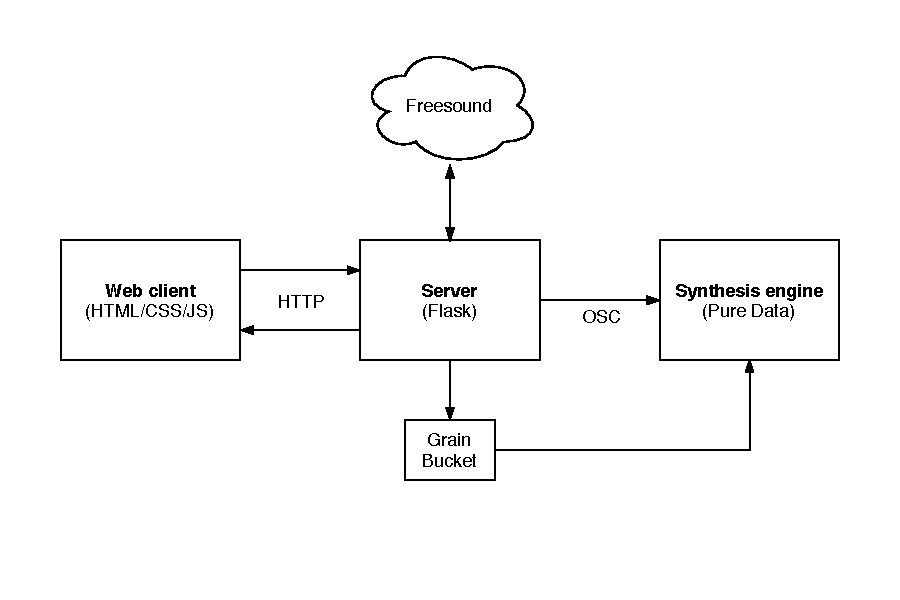
\includegraphics[width=\linewidth]{../img/granabular-system.pdf}
	\caption{System block diagram.}
	\centering
\end{figure}

\subsection{Synthesis engine}

The synthesis engine implements a fairly standard granular synthesizer. 
It features up to 32 simultaneous voices and supports the sourcing of grains
from a single source file at any given time. 
An implementation of freeverb\footnote{https://ccrma.stanford.edu/~jos/pasp/Freeverb.html} 
is included to provide artificial reverberation effects within the synthesizer. 

There are six main controls of the synthesizer as described in the list below, 
which are also shown within the user interface in Figure \ref{fig:engine}.

\begin{itemize}
	\item density: rate at which new grains are triggered
	\item start: position in the source file for grains
	\item pitch: the relative pitch of the 
	\item size: length of the grains
	\item start spray: degree of variation in starting position
	\item pan spray: degree of variation in spatialisation
\end{itemize}

The general operation of the synthesis is as follows. 
On every \emph{bang} produced by the main clock (whose rate is defined
by the density control), a grain is generated by selecting a starting sample 
from within the source file. This position is determined by the value of the 
start parameter. The starting sample is then modified to be earlier or later
by a number sampled from a gaussian with mean 0 and variance set with the start spray control.
This behaviour enables the grains to be sourced from slightly different starting positions
within the source file each time, which helps to reduce unwanted phasing artifacts.

\begin{figure}[h] \label{fig:engine}
	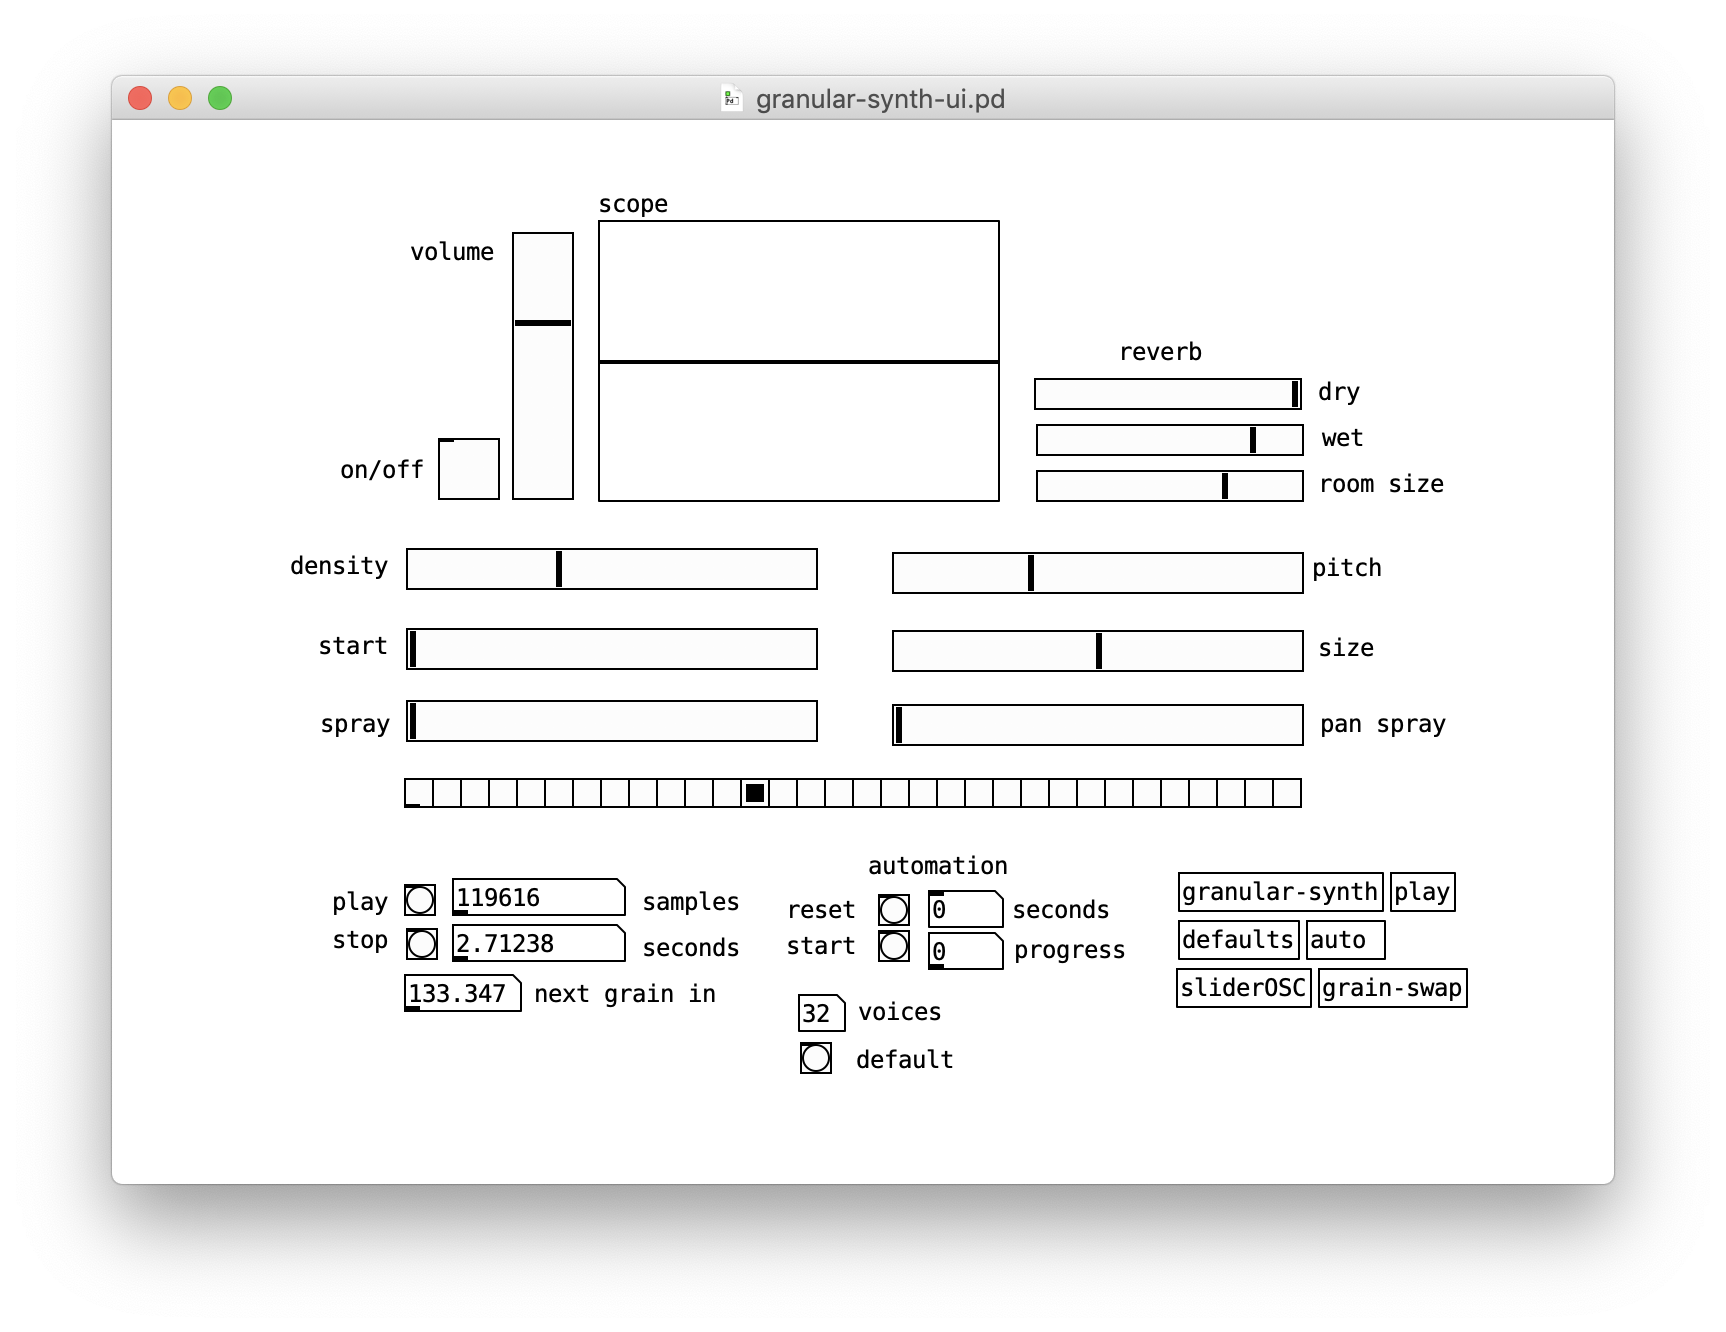
\includegraphics[width=\linewidth]{../img/engine.png}
	\caption{Granular synthesizer user interface.}
	\centering
\end{figure}

Once the starting position has been identified, the end of the grain is set
based upon the size parameter. A large size value means a longer grain and vice versa. 
With the current grain identified, a Hann window is applied to smooth any discontinuities at the beginning and end.
The pitch parameter then controls the rate at which this grain is played back. Finally, since all grains are
mono, they must be panned within the stereo field. By default the grain will play back equally in the left and right channels.
The pan spray control allows for the position of each grain to be determined randomly, and a greater value will mean 
the stereo field will be filled more widely. 

In order to provide diversity in the performance, multiple different source files will be used for grain generation. 
As described in the following section there are two methods for user's to generate these files. 
Once they are generated they will be placed in what is known the the \emph{grain bucket}, a list of all the files
as well as the path to their location. 
Within the synthesizer there is another clock which at random intervals 
will swap the current source file to another source file within the grain bucket. 
Therefore, as the number of source files grows, the possible diversity in performance grows as wel..

\subsection{Web client}

In order to provide an interface to control parameters of the synthesis engine, users can connect with the front-end web client. 
This is a simple web page which can be loaded on any device with a compatible web browser, such as a laptop of mobile phone. 
Since all of the content is provided via the web server (as will be addressed in the next section),
there is no installation process required for the end users. Users must simply be connected to the 
same network as the web server and then navigate to the proper address, where they will be prompted to join the session. 

\begin{figure}[hbt!] \label{fig:controller}
	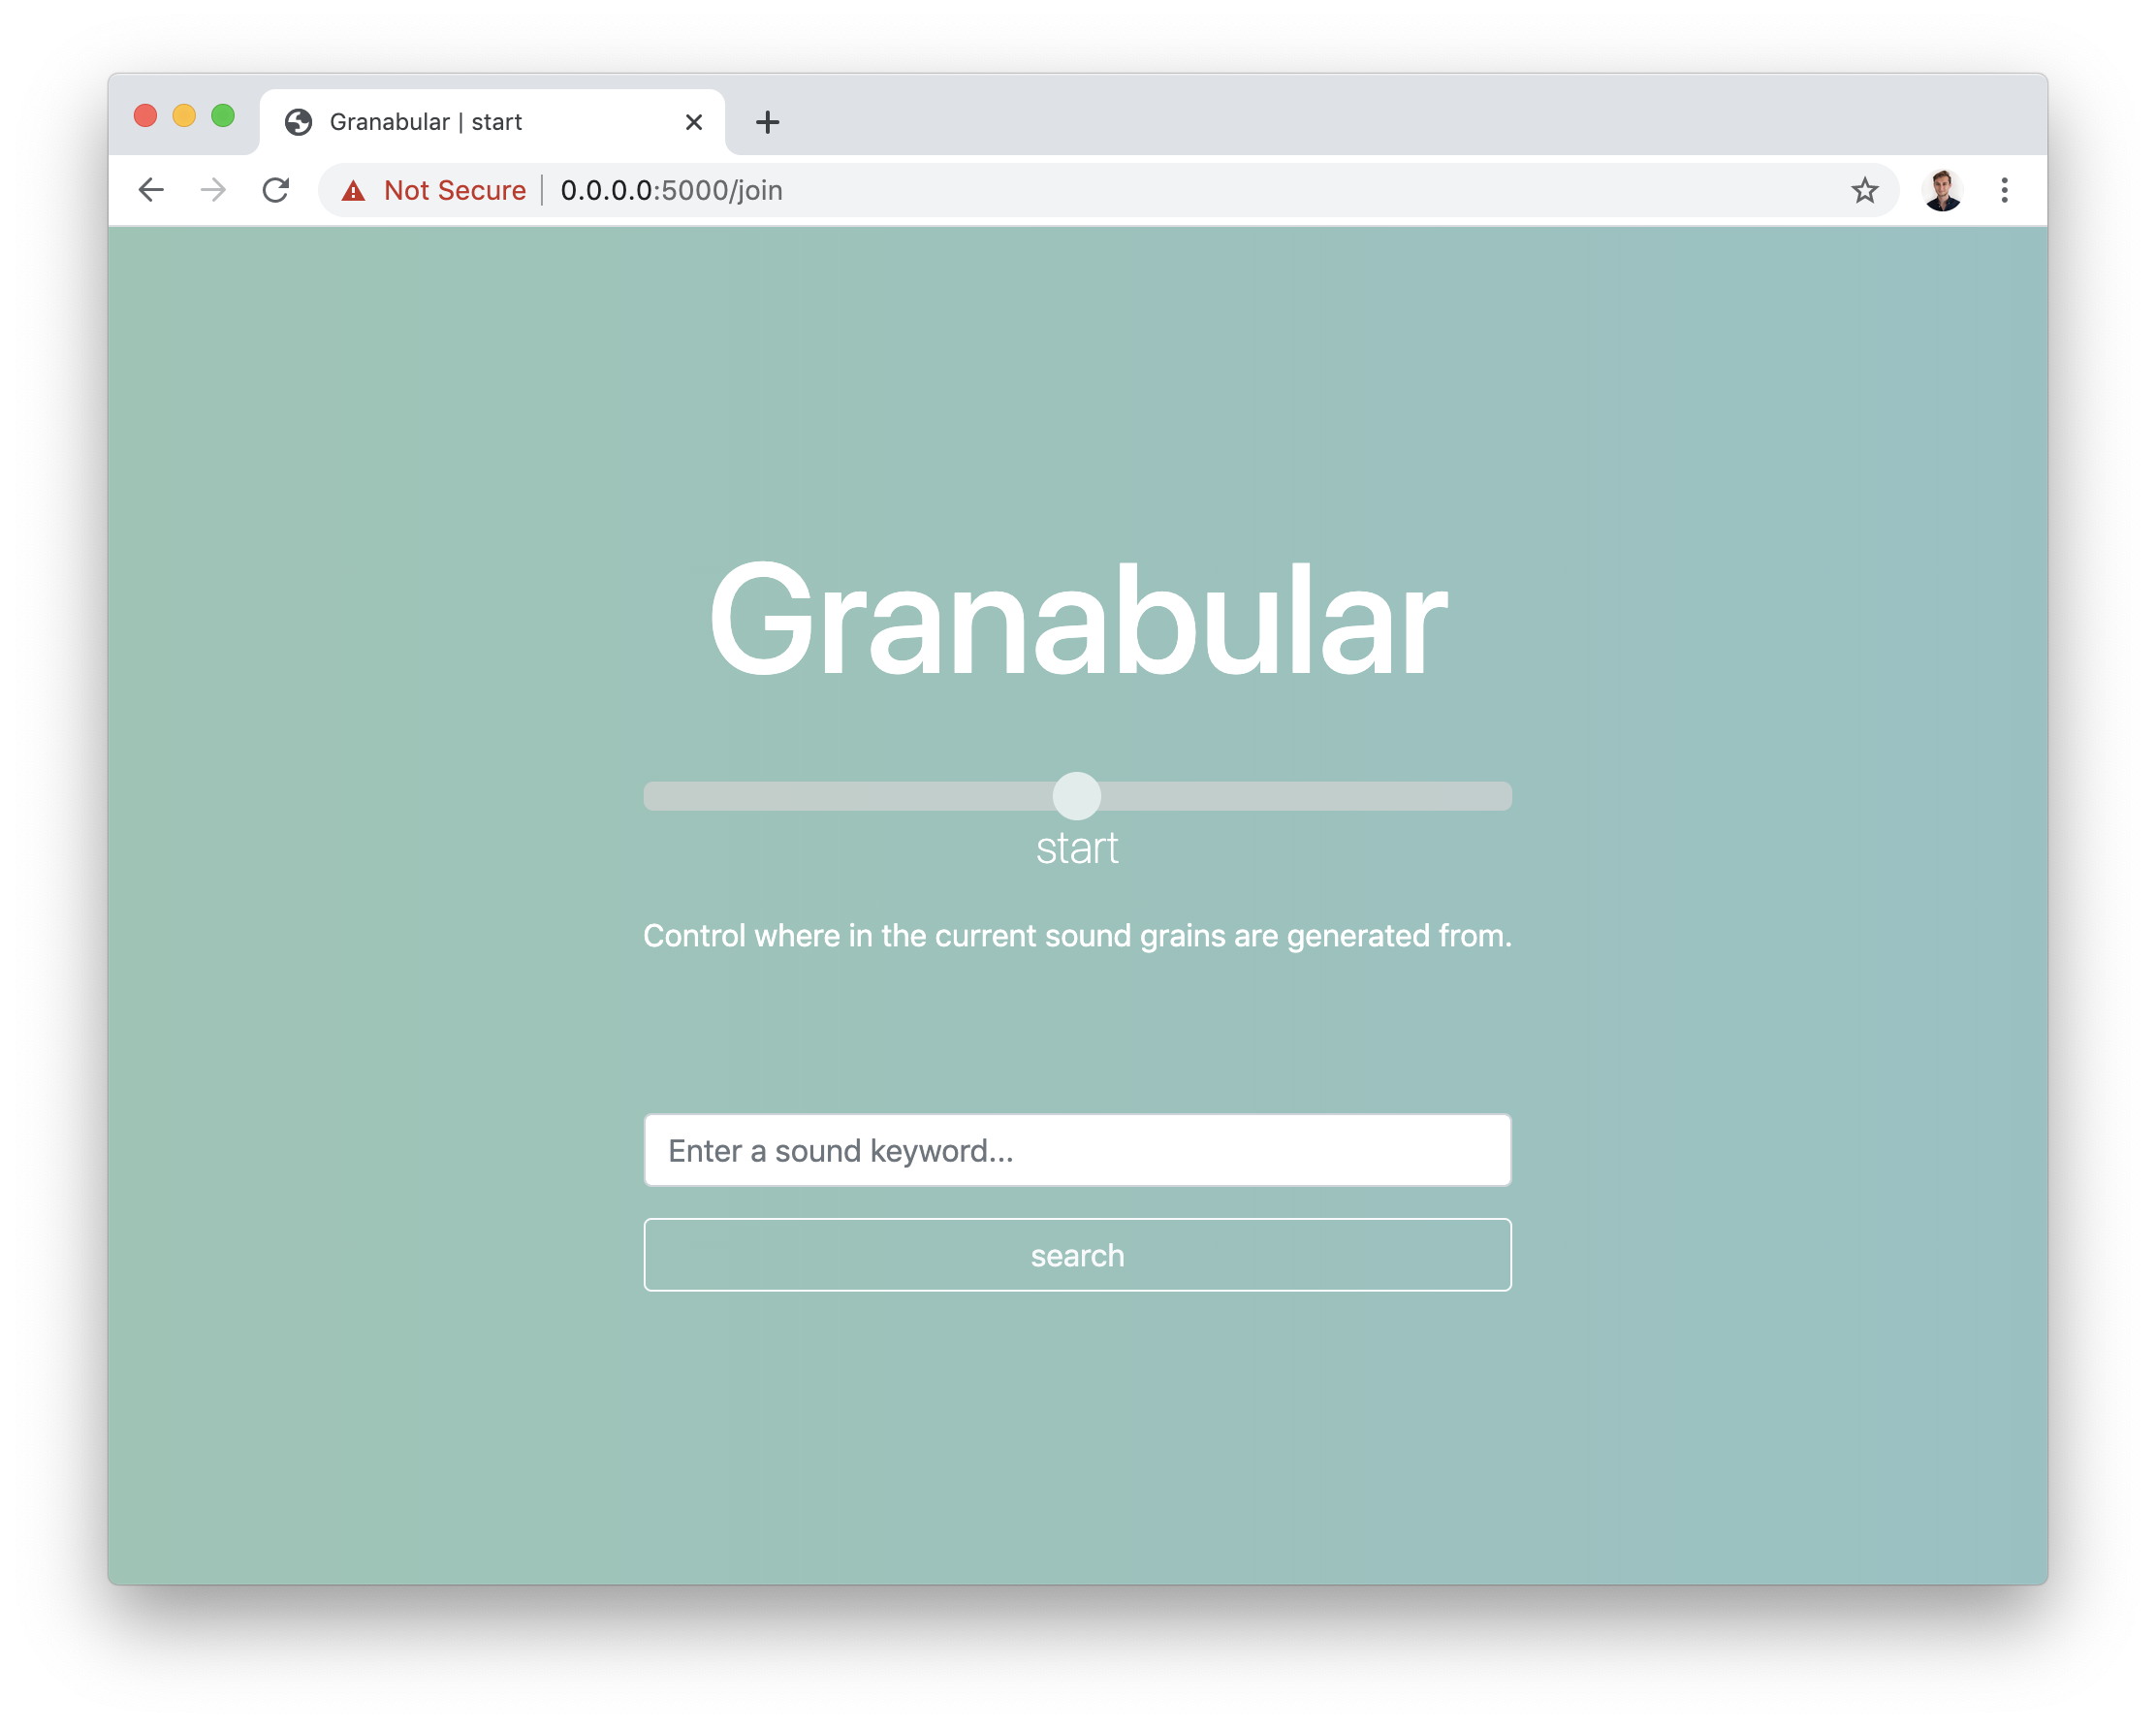
\includegraphics[width=\linewidth]{../img/controller.png}
	\caption{Minimalist browser-based client interface.}
	\centering
\end{figure}

After joining the current session, the user will be assigned one of the parameters of the synthesizer
at random, as shown in Figure \ref{fig:controller}. The interface is kept purposefully simple so as not 
to produce unnecessarily complexity. A single, large slider is placed in the center of the screen
as well as a simple description of its function. This interface remains approachable, even to novice users,
since they can simply experiment by moving the slider to build an intuitive understanding of its function. 

There are two main methods of generating source files to be used in the granular synthesis engine, both of which are user driven.
The first method involves directly recording source files via the microphone present in the user's device. 
If this mode is activated, when the user joins the session they will be prompted by their browser to allow access to their microphone.
If granted, at random intervals the interface will change color and indicate to the user that they should begin making noise as shown in Figure \ref{fig:recording}.
During this period of ten seconds a recording will be made with their device's microphone and it will then be sent to the web server. 

The second method involves sourcing recordings directly from Freesound\footnote{https://freesound.org/}, 
a platform for sharing creative commons recordings. 
In addition to the single range slider, users are also presented with an input box. 
They can type queries here which will then be sent to the server. The server will then send these queries to the Freesound API and download relevant files.
This modality provides a means to populate the \emph{grain bucket} without the need for the performers to generate any sounds themselves. 
The configuration in which device microphones are utilized is envisioned to function well with a group of performers who have with them
their own instruments or sound creation devices, which they can play during the recording period. Otherwise, this query driven method
for populating the \emph{grain bucket} provides a more convenient method. 

Since there are six main controls of the synthesizer, only six participants may join a session at any given time.
This ensures that only one users controls each parameter of the synthesizer. 
If additional users attempt to join a session they will see a message indicating that the current session is full.

\begin{figure}[h] \label{fig:recording}
	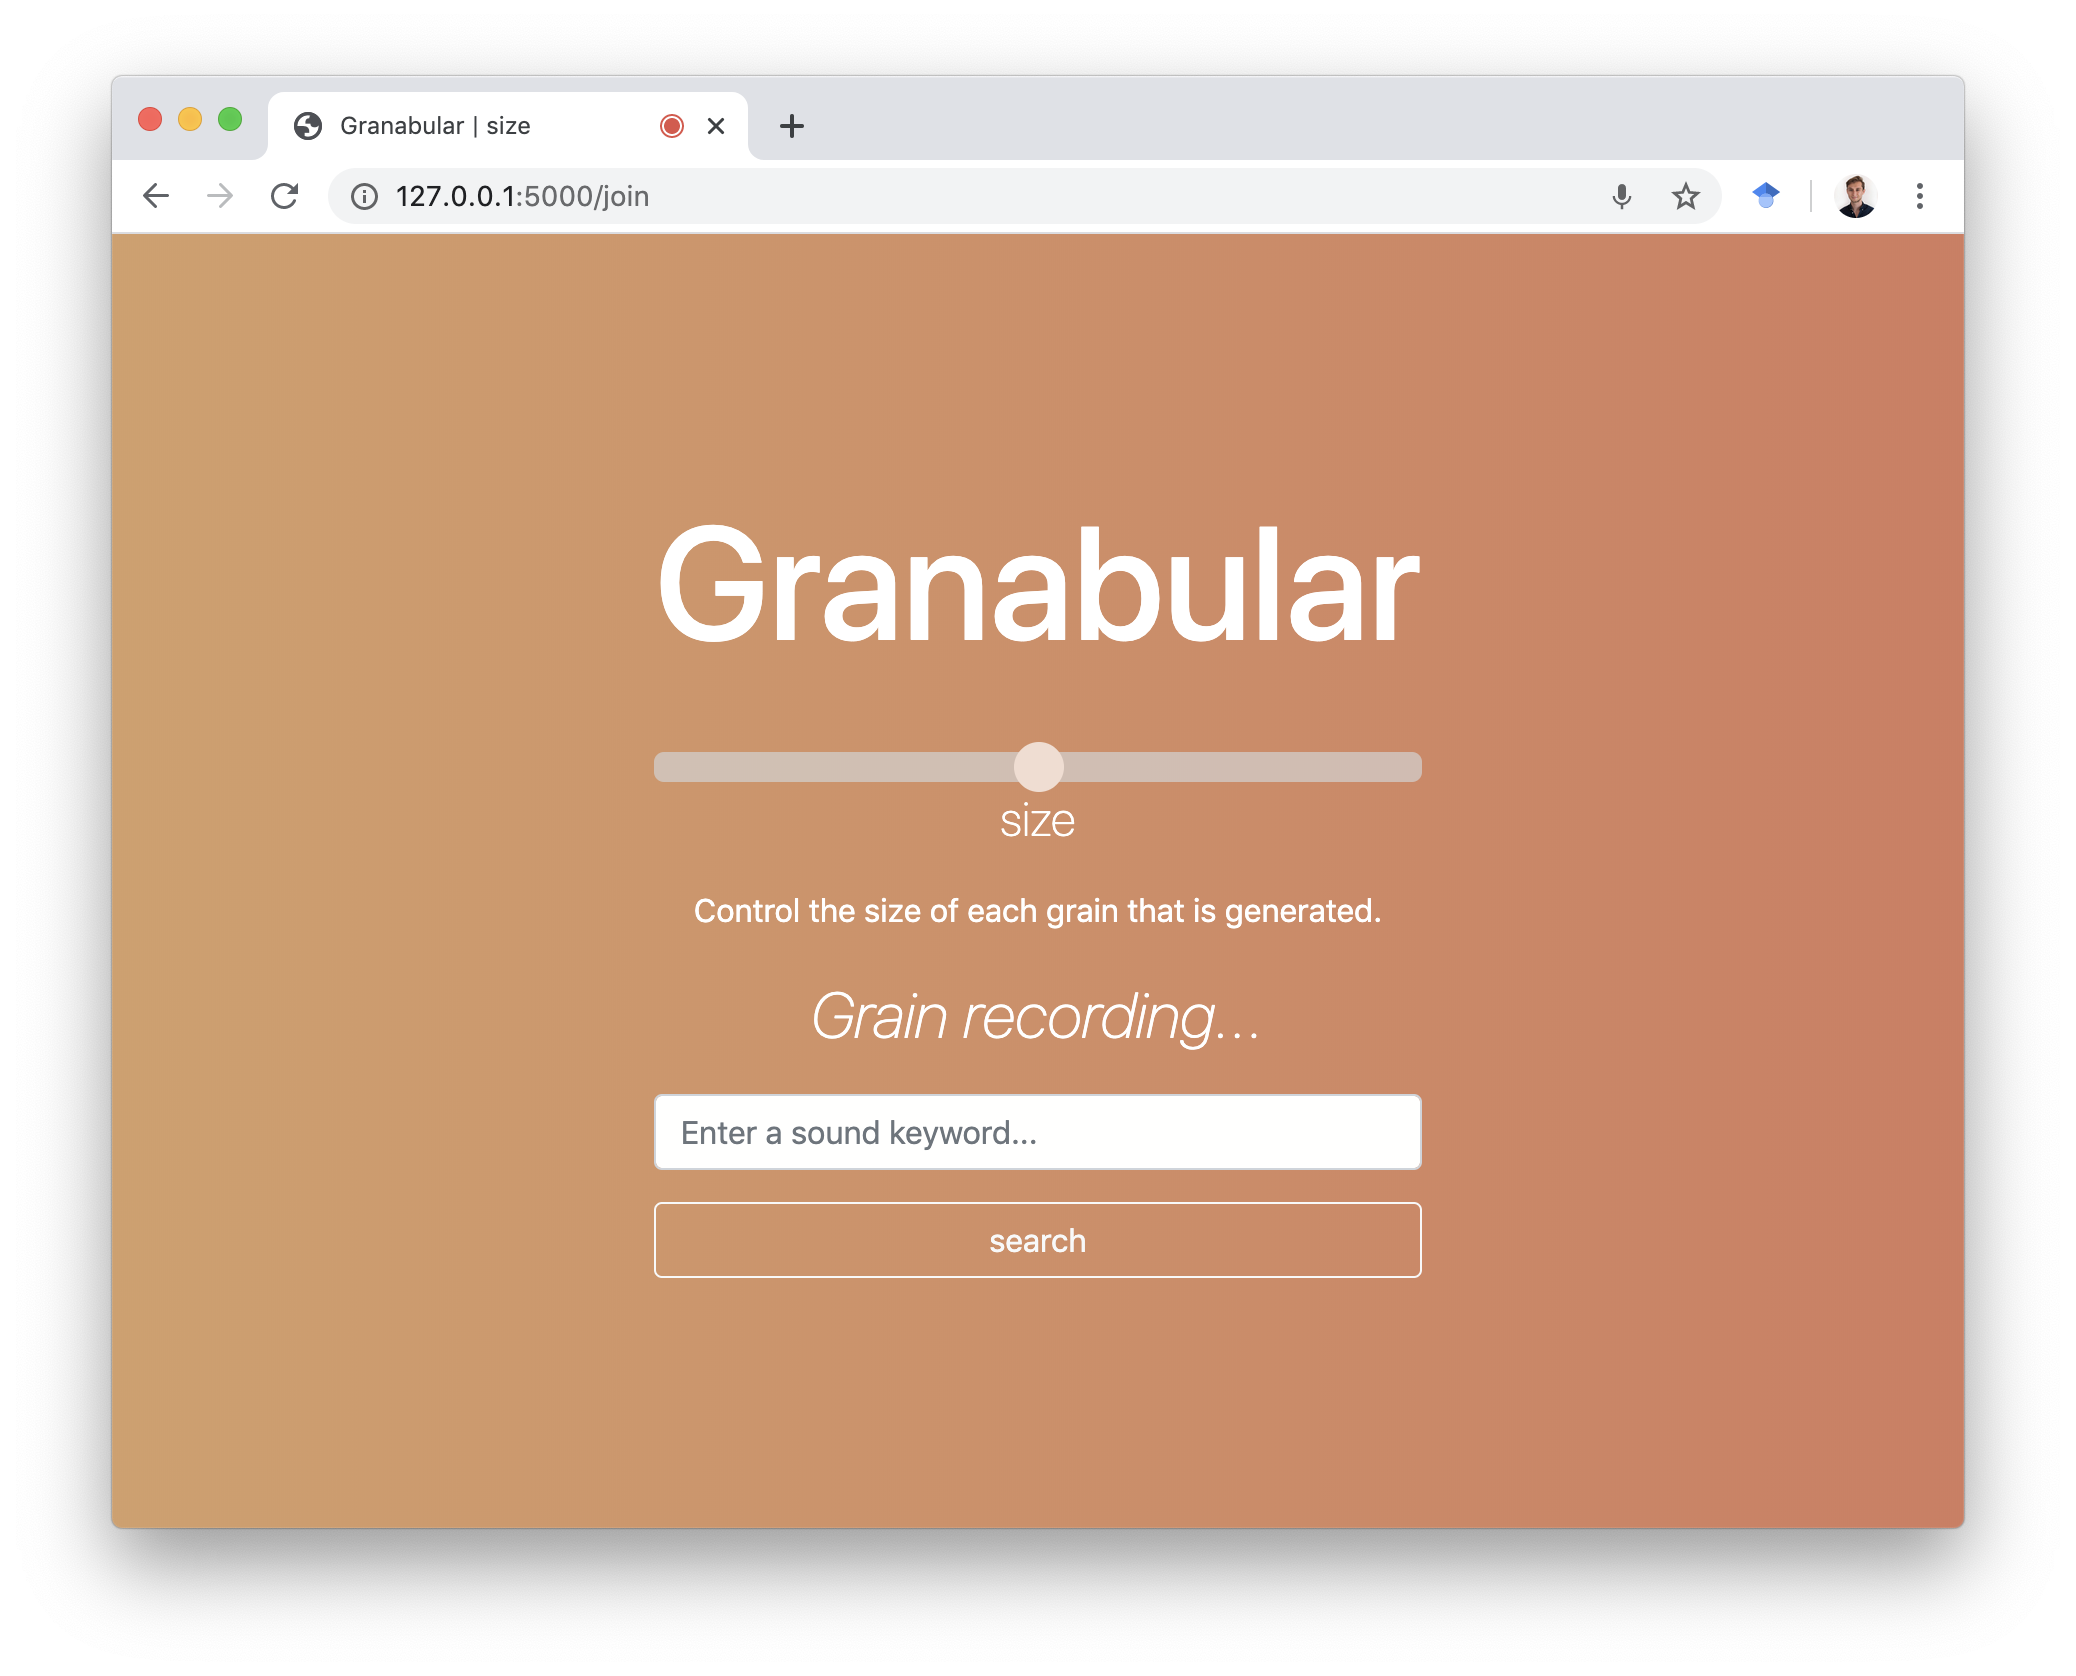
\includegraphics[width=\linewidth]{../img/recording.png}
	\caption{Active source file recording on the client.}
	\centering
\end{figure}

\subsection{Web server}

The web server functions as the main intermediary between the synthesis engine and the web client.
As shown in Figure \ref{fig:block-diagram}, POST and GET requests over HTTP are used for communication between the web server and the client,
and OSC (open sound control) messages are used to communicate the Pure data patch. 
An event listener responds whenever the user changes the slider and this sends a POST request to the server with the current value.
The server then relays this information to Pure data by sending an appropriate OSC message. 

When the user submits a search query, this string is sent to the web server, which then uses the Freesound API in order to find candidate recordings. 
A recording is selected at random from this list, it is then downloaded, converted to a to the WAV format at 16 bit 44.1 kHz using FFmpeg\footnote{https://www.ffmpeg.org/}, 
and finally an OSC message is sent to the patch to inform it of the location of the latest addition to the \emph{grain bucket}.
In a similar fashion, once a recording has been made with the user's microphone, it is sent to the server, converted, and it's location forwarded onto the patch.
In the case of recordings made from user microphones, a bit of extra processing is performed. 
First we measure the total amount of energy in the recording, and if it is below a set threshold we reject the recording, indicating it was mostly silence. 
If the recording does in fact contain significant signal we then peak normalize the recording so as to ensure it is loud enough on playback.

\section{Future work}

Granabular serves as an early prototype of the idea for a collaborative granular synthesizer.
For that reason there are a number of ways in which to extend or make the system more robust.
Additionally this prototype has been demonstrated in a live, multi-user performance, and
from this early experiment a number of areas of improvement have been additionally identified. 

One of the known limitations comes from the structure of the communication between the client 
and the server. Currently simple HTTP GET and POST requests are used. 
While these method work they do not allow for continuous communication between the systems.
To improve this we propose to use web sockets which would allow for continuous communication.
This could potentially lower latency in parameter control and also allow for the server to 
identify when a user has disconnected (closed the browser) so as to open this slot of the session to new users. 

Another improvement could be made by apply pre-processing to the parameter control signals. 
Currently whenever a slider is adjusted the instantaneous value is sent to the synthesizer. 
This can often cause in wanted effects if there is a lag in communication, resulting in a jerking sound.
Simply applying a filter to reduce the rate at which such parameter can be adjusted would help to 
alleviate this issue. 

Finally, additional post-processing could be performed to the recordings downloaded from Freesound.
During our demonstration, we found that many recordings downloaded included large sections of silence.
Simple post processing could be used to delete regions of silence to ensure that the source files
used in the synthesizer contain audible content at all times. 

\section{Conclusions}

A multi-user collaborative granular synthesizer system was proposed, which features two 
unique methods for generating source files in the synthesis process. 
Our system fosters collaboration between participants to construct evolving soundscapes
using a single granular synthesis engine. 
The client facing interface has been designed following minimalist principles in order to
facilitate participation from both experienced and novice users alike.  
We demonstrated the operation of this system in an interactive performance where multiple
users connected to the system and concurrently controlled different parameters of the synthesizer
to successfully generate an acoustic experience.

%ACKNOWLEDGMENTS are optional
%\section{Acknowledgments}

% The following two commands are all you need in the
% initial runs of your .tex file to
% produce the bibliography for the citations in your paper.
\bibliographystyle{abbrv}
\bibliography{nime-references}  % sigproc.bib is the name of the Bibliography in this case
% You must have a proper ".bib" file
%  and remember to run:
% latex bibtex latex latex
% to resolve all references
%
% ACM needs 'a single self-contained file'!
%

\end{document}
